\documentclass[11pt,a4paper]{article}
\usepackage[utf8]{inputenc}
\usepackage[T1]{fontenc}
\IfFileExists{french.ldf}{\usepackage[french]{babel}}{\usepackage[english]{babel}}
\usepackage{amsmath,amssymb}
\usepackage[margin=2.4cm]{geometry}
\usepackage{listings}
\usepackage{xcolor}
\usepackage{enumitem}
\usepackage{tikz}
\usepackage{titlesec}
\usepackage{fancyhdr}
\usepackage{hyperref}
\hypersetup{colorlinks=true, urlcolor=[RGB]{2,101,115}, linkcolor=black}
\definecolor{teal}{RGB}{2,101,115}
\definecolor{codebg}{RGB}{247,249,251}
\definecolor{kw}{RGB}{175,45,45}
\definecolor{cmt}{RGB}{110,120,130}
\lstset{language=Python, backgroundcolor=\color{codebg}, basicstyle=\ttfamily\footnotesize,
  keywordstyle=\color{kw}\bfseries, commentstyle=\color{cmt}\itshape, frame=single,
  rulecolor=\color{gray!40}, columns=fullflexible, breaklines=true, showstringspaces=false,
  aboveskip=4pt, belowskip=4pt, extendedchars=true, inputencoding=utf8,
  literate={é}{{\'e}}1 {è}{{\`e}}1 {à}{{\`a}}1 {ê}{{\^e}}1 {î}{{\^i}}1 {ç}{{\c c}}1 {ô}{{\^o}}1 {É}{{\'E}}1}
\newcommand{\code}[1]{\lstinline!#1!}
\newcounter{tache}[section]
\newcommand{\T}[1][]{\refstepcounter{tache}\smallskip\par\noindent\textbf{Q\thesection.\thetache}~{\itshape#1}~}
\setlength{\parskip}{0.5em}\setlength{\parindent}{0pt}
\titlespacing*{\section}{0pt}{1.3em}{0.5em}
\titleformat*{\section}{\bfseries\color{teal}}
\pagestyle{fancy}\fancyhf{}
\lhead{\small Agrégation d'informatique --- épreuve blanche}\rhead{\small Arbres de Merkle \& Bitcoin}
\cfoot{\thepage}\renewcommand{\headrulewidth}{0.4pt}

\begin{document}

\begin{center}
{\large\bfseries Agrégation externe d'informatique --- Épreuve blanche}\\[3pt]
{\bfseries Arbres de Merkle et vérification légère dans Bitcoin}\\[2pt]
{\small\itshape Théorie, simulations et implémentations --- durée indicative~: 4 h}
\end{center}

\vspace{-0.2em}
\begin{center}\footnotesize
\fbox{\begin{minipage}{0.97\linewidth}
Cette épreuve alterne des \textbf{questions théoriques} (à démontrer), des \textbf{tâches
d'implémentation} (à programmer en Python~3, modules \texttt{hashlib}, \texttt{numpy}) et des
\textbf{expériences de simulation} (à mener et à commenter). \textbf{Aucune réponse n'est
fournie.} On attend un code lisible, testé, et une analyse (correction, complexité, sécurité,
convergence). Les signatures données fixent seulement les interfaces attendues.
\end{minipage}}
\end{center}

\section{Cadre : blocs, transactions et en-tête}

Une blockchain de type Bitcoin est une suite de \emph{blocs}. Chaque bloc contient une liste
ordonnée de \emph{transactions} $t_0,\dots,t_{n-1}$ et un \emph{en-tête} de taille fixe. L'en-tête
comporte notamment~: le haché de l'en-tête précédent, un \emph{condensé} des transactions appelé
\emph{racine de Merkle}, un horodatage, une \emph{cible} de difficulté et un entier libre, le
\emph{nonce}. La sécurité repose sur une fonction de hachage. Bitcoin utilise le \emph{double
SHA-256}
\[
  H(m) \;=\; \mathrm{SHA256}\bigl(\mathrm{SHA256}(m)\bigr) \in \{0,1\}^{256},
\]
que l'on manipulera sous forme d'objets \texttt{bytes} de longueur $32$. On identifie une
transaction $t_i$ à son \emph{identifiant} $\mathrm{txid}_i = H(t_i)$. Toutes les concaténations
$a\Vert b$ portent sur les octets bruts.

\textbf{Objectifs.} On cherchera systématiquement à~: (i) \emph{démontrer} les propriétés
annoncées~; (ii) \emph{implémenter} les fonctions spécifiées et les \emph{tester}~; (iii)
\emph{simuler} pour confronter la théorie à l'expérience. Les six parties sont largement
indépendantes~; on pourra les aborder dans l'ordre de son choix.

\section{Fonction de hachage : propriétés et collisions}

\begin{lstlisting}
def H(m: bytes) -> bytes:
    """Double SHA-256 : renvoie 32 octets. A implementer avec hashlib."""
    ...
\end{lstlisting}

\T[(implémentation)] Implémenter \code{H}. Écrire un test vérifiant le déterminisme
($H(m)=H(m)$) et l'effet d'avalanche (un bit modifié change massivement la sortie, mesuré par la
distance de Hamming moyenne sur $32$ octets).

\T[(théorie)] Montrer qu'une fonction $\{0,1\}^{*}\to\{0,1\}^{256}$ ne peut être injective, et
donc que des collisions existent. Expliquer en quoi la \emph{résistance aux collisions} est une
hypothèse \emph{calculatoire} et non un théorème.

\T[(théorie)] On modélise $H$ comme un tirage uniforme dans un ensemble à $M=2^{b}$ valeurs. On
tire $k$ valeurs indépendantes. Montrer que la probabilité d'absence de collision vérifie
$q_k=\prod_{i=0}^{k-1}(1-i/M)\le \exp(-k(k-1)/2M)$, et en déduire que le seuil de collision
probable est de l'ordre de $\sqrt{M}=2^{b/2}$. Commenter le choix $b=256$.

\T[(simulation)] Pour un hachage \emph{tronqué} à $b\in\{16,24,32\}$ bits (ne garder que les $b$
premiers bits de $H$), estimer par une méthode de Monte-Carlo le nombre moyen de tirages avant la
première collision, et confronter la mesure à la prédiction $\Theta(2^{b/2})$. Présenter les
résultats dans un tableau ou un graphique.

\T[(théorie)] Distinguer trois notions de sécurité d'une fonction de hachage~: \emph{résistance
à la préimage}, \emph{à la seconde préimage}, et \emph{aux collisions}. Ordonner ces propriétés
(laquelle implique laquelle~?) et préciser laquelle est requise pour la sécurité des preuves de
Merkle de la partie~4.

\section{Racine de Merkle d'un bloc}

La \emph{racine de Merkle} résume les $n$ transactions. On procède par niveaux~: partant de la
liste des $\mathrm{txid}_i$, on remplace chaque paire consécutive $(a,b)$ par $H(a\Vert b)$~; si un
niveau contient un nombre \emph{impair} d'éléments, on \textbf{duplique son dernier élément} avant
l'appariement (règle de Bitcoin). On s'arrête sur un unique haché, la racine.

\begin{center}
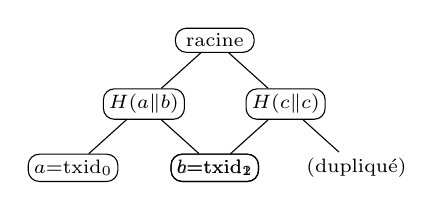
\begin{tikzpicture}[level distance=9mm, sibling distance=20mm, scale=0.9,
  every node/.style={draw,rounded corners,inner sep=2pt,font=\scriptsize,minimum width=10mm}]
\node {racine}
  child {node {$H(a\Vert b)$} child {node {$a{=}\mathrm{txid}_0$}} child {node {$b{=}\mathrm{txid}_1$}}}
  child {node {$H(c\Vert c)$} child {node {$c{=}\mathrm{txid}_2$}} child[draw=none] {node[draw=none]{\scriptsize(dupliqué)}}};
\end{tikzpicture}\\[-2pt]
{\footnotesize Figure~1 --- bloc à $3$ transactions~: le dernier haché est dupliqué.}
\end{center}

\begin{lstlisting}
def merkle_root(txids: list[bytes]) -> bytes:
    """Racine de Merkle (regle Bitcoin : duplication si niveau impair).
       Precondition : len(txids) >= 1."""
    ...
\end{lstlisting}

\T[(implémentation)] Implémenter \code{merkle_root}. Traiter correctement le cas $n=1$ et la
duplication. Tester sur des blocs de $1,2,3,4,5$ transactions.

\T[(théorie)] Soit $n$ le nombre de transactions. Montrer que le calcul de la racine effectue
$O(n)$ évaluations de $H$ et que la hauteur de l'arbre vaut $\lceil\log_2 n\rceil$. \emph{On
majorera la somme des tailles des niveaux successifs.}

\T[(théorie)] Décrire une conséquence de la règle de duplication en termes de sécurité~: montrer
qu'un bloc à nombre impair de transactions et un bloc obtenu en dupliquant réellement la dernière
transaction peuvent produire la \emph{même} racine (malléabilité de type \guillemotleft~CVE-2012-2459~\guillemotright). Que faut-il vérifier en plus de la racine~?

\section{Preuves de Merkle et vérification simplifiée (SPV)}

Un client \emph{léger} (\emph{Simplified Payment Verification}) ne stocke que les en-têtes des
blocs. Pour lui prouver qu'une transaction $t$ appartient à un bloc de racine $R$, on fournit une
\emph{preuve de Merkle}~: la liste des hachés \emph{frères} rencontrés en remontant de la feuille
$H(t)$ jusqu'à la racine, chacun muni de son côté (\texttt{'L'} ou \texttt{'R'}).

\begin{lstlisting}
def preuve_merkle(txids: list[bytes], i: int) -> list[tuple[bytes, str]]:
    """Chemin de freres (haché, cote) de la feuille i jusqu'a la racine."""
    ...
def verifier_preuve(feuille: bytes, preuve, racine: bytes) -> bool:
    """Recalcule la racine a partir de la feuille et de la preuve."""
    ...
\end{lstlisting}

\T[(implémentation)] Implémenter \code{preuve_merkle} et \code{verifier_preuve}. Vérifier, sur un
bloc aléatoire de $n$ transactions, que toute transaction présente est acceptée, et qu'une
transaction absente (ou une preuve altérée) est rejetée.

\T[(théorie)] Montrer que la taille d'une preuve d'inclusion est $O(\log n)$. Comparer, pour
$n=10^{4}$ transactions, au coût de télécharger le bloc entier~; justifier l'intérêt du modèle SPV.

\T[(théorie)] \emph{Sécurité (soundness).} Démontrer, par récurrence sur la hauteur de l'arbre et
sous l'hypothèse de résistance aux collisions de $H$, que si \code{verifier_preuve} accepte une
feuille pour la racine authentique $R$, alors --- sauf à exhiber une collision de $H$ --- cette
feuille figure réellement parmi les transactions du bloc. Expliciter la \emph{réduction}~: comment
une fausse preuve fournit-elle algorithmiquement une collision~?

\T[(simulation)] Mesurer empiriquement la taille moyenne des preuves (nombre de frères) en
fonction de $n$ pour $n=2^{j}$, $j=1,\dots,14$, et confronter à $\lceil\log_2 n\rceil$. Tracer le
résultat.

\T[(implémentation)] Un message \texttt{merkleblock} de Bitcoin transmet, en une seule fois, les
preuves d'inclusion de \emph{plusieurs} transactions d'intérêt à l'aide d'un \emph{arbre de Merkle
partiel} (les sous-arbres ne contenant aucune transaction d'intérêt sont remplacés par leur seul
haché racine). Spécifier puis implémenter une fonction \code{arbre_partiel(txids, indices)} qui
produit un tel certificat compact, et \code{verifier_partiel} qui le valide. Comparer sa taille à
la somme des preuves individuelles.

\section{Preuve de travail (minage)}

L'en-tête $e$ contient un \emph{nonce} $\nu$. \emph{Miner} le bloc, c'est trouver $\nu$ tel que
$H(e_\nu)$, interprété comme un entier sur $256$ bits, soit strictement inférieur à une
\emph{cible} $T$. On note $p=T/2^{256}$ la probabilité, pour un essai, de satisfaire la condition
(modèle de l'oracle aléatoire).

\begin{lstlisting}
def mine(entete_sans_nonce: bytes, cible_bits_zero: int) -> tuple[int, bytes]:
    """Cherche le plus petit nonce (32 bits, big-endian concatene) tel que
       H(entete || nonce) commence par 'cible_bits_zero' bits a zero.
       Renvoie (nonce, hache). Ici la cible T = 2**(256 - cible_bits_zero)."""
    ...
\end{lstlisting}

\T[(implémentation)] Implémenter \code{mine} en exigeant $k$ bits de tête nuls (donc $p=2^{-k}$).
La tester pour $k$ croissant et relever le nombre d'essais.

\T[(théorie)] Soit $N$ le nombre d'essais jusqu'au premier succès. Donner la loi de $N$, montrer
que $\mathbb{E}[N]=1/p=2^{k}$ et que le minage \emph{termine presque sûrement}
($\mathbb{P}(N=\infty)=0$). Ce processus est-il un algorithme au sens usuel~? Discuter la notion
de \emph{terminaison probabiliste}.

\T[(simulation)] Pour $k\in\{8,12,16,20\}$, estimer $\mathbb{E}[N]$ par Monte-Carlo (moyenne sur
plusieurs minages indépendants) et comparer à $2^{k}$. Tracer l'histogramme empirique de $N$ pour
un $k$ fixé et vérifier qu'il épouse une loi géométrique (décroissance de raison $1-p$).

\T[(théorie \& simulation)] Bitcoin ajuste périodiquement la cible pour maintenir un temps moyen
entre blocs constant, malgré une puissance de calcul $\lambda$ (hachages par seconde) variable.
En supposant $N$ géométrique et $\lambda$ constant sur la période, exprimer le temps moyen d'un
bloc en fonction de $p$ et $\lambda$, puis proposer une règle d'ajustement de $T$ lorsque
$\lambda$ double. Illustrer par une simulation où $\lambda$ varie par paliers.

\T[(théorie \& simulation)] \emph{Course entre chaînes.} Un attaquant disposant d'une fraction
$\alpha<1/2$ de la puissance de calcul tente de rattraper la chaîne honnête partie avec $z$ blocs
d'avance. En modélisant l'écart de blocs par une marche aléatoire, estimer par simulation la
probabilité de rattrapage en fonction de $\alpha$ et $z$, et observer sa décroissance exponentielle
en $z$. Relier au principe de \emph{confirmation} (attendre $z$ blocs avant de considérer une
transaction comme définitive).

\section*{Prolongements (facultatifs)}
\begin{itemize}[nosep,leftmargin=1.2em]
  \item Comparer l'arbre de Merkle binaire de Bitcoin à l'arbre de \emph{Patricia-Merkle}
        d'Ethereum et aux \emph{arbres de Verkle} (taille de preuve $O(1)$).
  \item Étudier la complexité et la sécurité d'une mise à jour dynamique de la racine lorsqu'une
        transaction change ($O(\log n)$).
  \item Relier la résistance aux collisions aux \emph{fonctions à sens unique} et au cadre de la
        cryptographie à sécurité prouvée.
\end{itemize}

\section*{Références}
\begin{enumerate}[nosep,leftmargin=1.5em]
  \item S.~Nakamoto, \emph{Bitcoin: A Peer-to-Peer Electronic Cash System}, 2008 (sections
        \guillemotleft~Merkle Tree~\guillemotright{} et \guillemotleft~Calculations~\guillemotright).
  \item R.~C.~Merkle, \emph{A digital signature based on a conventional encryption function},
        CRYPTO~'87.
  \item A.~M.~Antonopoulos, \emph{Mastering Bitcoin}, O'Reilly~; A.~M.~Antonopoulos, G.~Wood,
        \emph{Mastering Ethereum}, O'Reilly.
  \item J.~Katz, Y.~Lindell, \emph{Introduction to Modern Cryptography}, CRC Press.
\end{enumerate}

\vspace{0.4em}
\hrule\smallskip
{\footnotesize\itshape Épreuve blanche (énoncé seul, sans corrigé) --- Pr Agrégé El Hadiq Zouhair,
\href{https://cpgeacademy.org}{cpgeacademy.org}.}

\end{document}
